% Options for packages loaded elsewhere
% Options for packages loaded elsewhere
\PassOptionsToPackage{unicode}{hyperref}
\PassOptionsToPackage{hyphens}{url}
\PassOptionsToPackage{dvipsnames,svgnames,x11names}{xcolor}
%
\documentclass[
  letterpaper,
  DIV=11,
  numbers=noendperiod]{scrartcl}
\usepackage{xcolor}
\usepackage{amsmath,amssymb}
\setcounter{secnumdepth}{5}
\usepackage{iftex}
\ifPDFTeX
  \usepackage[T1]{fontenc}
  \usepackage[utf8]{inputenc}
  \usepackage{textcomp} % provide euro and other symbols
\else % if luatex or xetex
  \usepackage{unicode-math} % this also loads fontspec
  \defaultfontfeatures{Scale=MatchLowercase}
  \defaultfontfeatures[\rmfamily]{Ligatures=TeX,Scale=1}
\fi
\usepackage{lmodern}
\ifPDFTeX\else
  % xetex/luatex font selection
\fi
% Use upquote if available, for straight quotes in verbatim environments
\IfFileExists{upquote.sty}{\usepackage{upquote}}{}
\IfFileExists{microtype.sty}{% use microtype if available
  \usepackage[]{microtype}
  \UseMicrotypeSet[protrusion]{basicmath} % disable protrusion for tt fonts
}{}
\makeatletter
\@ifundefined{KOMAClassName}{% if non-KOMA class
  \IfFileExists{parskip.sty}{%
    \usepackage{parskip}
  }{% else
    \setlength{\parindent}{0pt}
    \setlength{\parskip}{6pt plus 2pt minus 1pt}}
}{% if KOMA class
  \KOMAoptions{parskip=half}}
\makeatother
% Make \paragraph and \subparagraph free-standing
\makeatletter
\ifx\paragraph\undefined\else
  \let\oldparagraph\paragraph
  \renewcommand{\paragraph}{
    \@ifstar
      \xxxParagraphStar
      \xxxParagraphNoStar
  }
  \newcommand{\xxxParagraphStar}[1]{\oldparagraph*{#1}\mbox{}}
  \newcommand{\xxxParagraphNoStar}[1]{\oldparagraph{#1}\mbox{}}
\fi
\ifx\subparagraph\undefined\else
  \let\oldsubparagraph\subparagraph
  \renewcommand{\subparagraph}{
    \@ifstar
      \xxxSubParagraphStar
      \xxxSubParagraphNoStar
  }
  \newcommand{\xxxSubParagraphStar}[1]{\oldsubparagraph*{#1}\mbox{}}
  \newcommand{\xxxSubParagraphNoStar}[1]{\oldsubparagraph{#1}\mbox{}}
\fi
\makeatother


\usepackage{longtable,booktabs,array}
\newcounter{none} % for unnumbered tables
\usepackage{calc} % for calculating minipage widths
% Correct order of tables after \paragraph or \subparagraph
\usepackage{etoolbox}
\makeatletter
\patchcmd\longtable{\par}{\if@noskipsec\mbox{}\fi\par}{}{}
\makeatother
% Allow footnotes in longtable head/foot
\IfFileExists{footnotehyper.sty}{\usepackage{footnotehyper}}{\usepackage{footnote}}
\makesavenoteenv{longtable}
\usepackage{graphicx}
\makeatletter
\newsavebox\pandoc@box
\newcommand*\pandocbounded[1]{% scales image to fit in text height/width
  \sbox\pandoc@box{#1}%
  \Gscale@div\@tempa{\textheight}{\dimexpr\ht\pandoc@box+\dp\pandoc@box\relax}%
  \Gscale@div\@tempb{\linewidth}{\wd\pandoc@box}%
  \ifdim\@tempb\p@<\@tempa\p@\let\@tempa\@tempb\fi% select the smaller of both
  \ifdim\@tempa\p@<\p@\scalebox{\@tempa}{\usebox\pandoc@box}%
  \else\usebox{\pandoc@box}%
  \fi%
}
% Set default figure placement to htbp
\def\fps@figure{htbp}
\makeatother


% definitions for citeproc citations
\NewDocumentCommand\citeproctext{}{}
\NewDocumentCommand\citeproc{mm}{%
  \begingroup\def\citeproctext{#2}\cite{#1}\endgroup}
\makeatletter
 % allow citations to break across lines
 \let\@cite@ofmt\@firstofone
 % avoid brackets around text for \cite:
 \def\@biblabel#1{}
 \def\@cite#1#2{{#1\if@tempswa , #2\fi}}
\makeatother
\newlength{\cslhangindent}
\setlength{\cslhangindent}{1.5em}
\newlength{\csllabelwidth}
\setlength{\csllabelwidth}{3em}
\newenvironment{CSLReferences}[2] % #1 hanging-indent, #2 entry-spacing
 {\begin{list}{}{%
  \setlength{\itemindent}{0pt}
  \setlength{\leftmargin}{0pt}
  \setlength{\parsep}{0pt}
  % turn on hanging indent if param 1 is 1
  \ifodd #1
   \setlength{\leftmargin}{\cslhangindent}
   \setlength{\itemindent}{-1\cslhangindent}
  \fi
  % set entry spacing
  \setlength{\itemsep}{#2\baselineskip}}}
 {\end{list}}
\usepackage{calc}
\newcommand{\CSLBlock}[1]{\hfill\break\parbox[t]{\linewidth}{\strut\ignorespaces#1\strut}}
\newcommand{\CSLLeftMargin}[1]{\parbox[t]{\csllabelwidth}{\strut#1\strut}}
\newcommand{\CSLRightInline}[1]{\parbox[t]{\linewidth - \csllabelwidth}{\strut#1\strut}}
\newcommand{\CSLIndent}[1]{\hspace{\cslhangindent}#1}



\setlength{\emergencystretch}{3em} % prevent overfull lines

\providecommand{\tightlist}{%
  \setlength{\itemsep}{0pt}\setlength{\parskip}{0pt}}



 


\KOMAoption{captions}{tableheading}
\makeatletter
\@ifpackageloaded{caption}{}{\usepackage{caption}}
\AtBeginDocument{%
\ifdefined\contentsname
  \renewcommand*\contentsname{Table of contents}
\else
  \newcommand\contentsname{Table of contents}
\fi
\ifdefined\listfigurename
  \renewcommand*\listfigurename{List of Figures}
\else
  \newcommand\listfigurename{List of Figures}
\fi
\ifdefined\listtablename
  \renewcommand*\listtablename{List of Tables}
\else
  \newcommand\listtablename{List of Tables}
\fi
\ifdefined\figurename
  \renewcommand*\figurename{Figure}
\else
  \newcommand\figurename{Figure}
\fi
\ifdefined\tablename
  \renewcommand*\tablename{Table}
\else
  \newcommand\tablename{Table}
\fi
}
\@ifpackageloaded{float}{}{\usepackage{float}}
\floatstyle{ruled}
\@ifundefined{c@chapter}{\newfloat{codelisting}{h}{lop}}{\newfloat{codelisting}{h}{lop}[chapter]}
\floatname{codelisting}{Listing}
\newcommand*\listoflistings{\listof{codelisting}{List of Listings}}
\makeatother
\makeatletter
\makeatother
\makeatletter
\@ifpackageloaded{caption}{}{\usepackage{caption}}
\@ifpackageloaded{subcaption}{}{\usepackage{subcaption}}
\makeatother
\usepackage{bookmark}
\IfFileExists{xurl.sty}{\usepackage{xurl}}{} % add URL line breaks if available
\urlstyle{same}
\hypersetup{
  pdftitle={Fear of the invader: a predatory invader may provoke stronger non-consumptive effects on a keystone native prey than a co-evolved native predator},
  pdfauthor={Olivier V. Raven; Calum MacNeil; Finnbar Lee; Robin Holmes; Ian A. Kusabs; Francis J. Burdon; Deniz Özkundakci},
  pdfkeywords={Non-consumptive effects, Crayfish, Kōura, Brown bullhead
catfish, Antipredator behaviour},
  colorlinks=true,
  linkcolor={blue},
  filecolor={Maroon},
  citecolor={Blue},
  urlcolor={Blue},
  pdfcreator={LaTeX via pandoc}}


\title{Fear of the invader: a predatory invader may provoke stronger
non-consumptive effects on a keystone native prey than a co-evolved
native predator}
\author{Olivier V. Raven \and Calum MacNeil \and Finnbar Lee \and Robin
Holmes \and Ian A. Kusabs \and Francis J. Burdon \and Deniz Özkundakci}
\date{2026-05-04}
\begin{document}
\maketitle
\begin{abstract}
Non-consumptive effects (NCEs) of predators on prey encompass costly
antipredator behaviours such as increased refuge use and reduced
foraging, which can influence prey population dynamics and community
structure, particularly when the prey themselves are keystone species.
In Aotearoa-New Zealand, the native freshwater crayfish kōura
(\emph{Paranephrops planifrons}) is a keystone species, an ecosystem
engineer with a critical functional role in sediment dynamics, nutrient
cycling and benthic community structure. Kōura are preyed upon by both
the co-evolved native longfin eel (\emph{Anguilla dieffenbachii}) and
invasive brown bullhead catfish (\emph{Ameiurus nebulosus}), a species
introduced less than two centuries ago. Under laboratory conditions, we
tested whether visual and chemical cues from these two predators induced
different refuge-seeking and feeding behaviour responses by kōura.
Predator presence produced a NCE on refuge use, with kōura exposed to
catfish cues showing significantly greater refuge-seeking behaviour than
those exposed to eel cues. This is consistent with the generalisation
theory triggered by unfamiliar predator cues rather than classic prey
naivety . Our study indicates catfish incursions may provoke a greater
NCEs on kōura refuge use than resident eels. As catfish range expansion
continues, these NCEs represent an ecologically significant and
underappreciated threat to kōura populations, compounding the direct
predation pressure already documented for this invader.
\end{abstract}

\renewcommand*\contentsname{Table of contents}
{
\setcounter{tocdepth}{3}
\tableofcontents
}

\section{Introduction}\label{introduction}

Biological invasions can have profound impacts on invaded ecosystems,
particularly through the introduction of novel predators that prey upon
native species lacking an evolutionary history with them
(\citeproc{ref-Doherty2016}{Doherty et al., 2016}). Native prey may be
naïve not just to a specific invader, but to entire functional groups of
predators, making them especially vulnerable to direct predation when an
invasion introduces a predator type entirely absent from their
evolutionary history {[}Sih2010; Carthey2014{]}. In addition to these
consumptive effects, native prey may exhibit heightened fear responses
to invasive predators, leading to the development of anti-predator
behaviours such as increased refuge use and avoidance of open habitats
(\citeproc{ref-Kindlinger2017}{Kindinger \& Albins, 2017}). These
behavioural changes, termed non-consumptive effects (NCEs), can
substantially influence population dynamics by reducing foraging
activity, growth, and reproductive output
(\citeproc{ref-Preisser2005}{Preisser et al., 2005}). In contrast,
native predators generally elicit different responses because prey and
predators have co-evolved, resulting in behavioural and physiological
adaptations that stabilise predator--prey interactions
(\citeproc{ref-Abrams2000}{Abrams, 2000}).

Freshwater crayfish often live in turbid flowing water or in the dark
depths of lakes where they rely primarily on chemical cues (kairomones)
rather than visual cues to detect and respond to predatory fish
(\citeproc{ref-Blake1993}{Blake \& Hart, 1993};
\citeproc{ref-Bronmark2012}{Brönmark \& Hansson, 2012};
\citeproc{ref-Wood2020b}{Wood \& Moore, 2020b}). These kairomones carry
signals via excreta, mucus, or skin, that crayfish use to assess
predator risk, responding more strongly to predators that have consumed
conspecifics and to alarm cues released when prey is injured or killed
(\citeproc{ref-Beattie2018}{Beattie \& Moore, 2018};
\citeproc{ref-Gherardi2011}{Gherardi et al., 2011}). Exposure to
kairomones from predatory fish can generate NCEs, including reduced
growth and reduced activity levels in crayfish
(\citeproc{ref-Adams2007}{Adams, 2007};
\citeproc{ref-RambergPihl2020}{Ramberg-Pihl \& Yurewicz, 2020}), and
even non-predatory fish can cause these behaviour changes, likely
through heightened generalised awareness of risk
(\citeproc{ref-Nystrom2005}{Nyström, 2005}). However, the strength of
these responses depends on prior experience as wild-caught individual
crayfish show stronger antipredator responses than farmed conspecifics
naive to predators (\citeproc{ref-Martin2014}{Martin, 2014}), indicating
that both learned behavior and evolutionary history shape kairomone
detection.

In Aotearoa-New Zealand (hereafter Aotearoa), the endemic northern
freshwater crayfish \emph{Paranephrops planifrons} (White, 1842)
commonly known as kōura is a taonga (`culturally treasured') species for
Māori, the indigenous people of Aotearoa and is valued as a food
resource (\citeproc{ref-Kusabs2009}{Kusabs \& Quinn, 2009}).
Ecologically, kōura play a critical role in freshwater ecosystems as
ecosystem engineers through their effects on sediment dynamics, nutrient
cycling, and benthic community structure, and have been described as
keystone species in many freshwater systems
(\citeproc{ref-Collier1997}{Collier et al., 1997};
\citeproc{ref-Parkyn2001}{Parkyn et al., 2001};
\citeproc{ref-Usio2004}{Usio \& Townsend, 2004}). Currently kōura are
threatened by multiple interacting stressors, including climate change,
water-quality degradation and invasive species, contributing to
widespread population declines (\citeproc{ref-Kusabsinrevision}{Kusabs
et al., n.d.}; \citeproc{ref-Lee2025}{Lee et al., 2025}).

Kōura have a long co-evolutionary history with the native longfin eel
(\emph{Anguilla dieffenbachii}) (hereafter eel) and shortfin eel
(\emph{A. australis}) (\citeproc{ref-Brown2009}{L. A. Brown, 2009};
\citeproc{ref-MacNeil2025}{MacNeil et al., 2025}). Reflecting this
history, kōura respond more strongly to eel kairomones than to those of
introduced non-native brown trout (\emph{Salmo trutta}), even when
sourced from streams where both predators were present, suggesting that
co-evolutionary history, rather than individual experience alone, shaped
kōura predator recognition (\citeproc{ref-Shave1994}{Shave et al.,
1994}). One of the invasive species that threatens kōura is the
non-native brown bullhead catfish (\emph{Ameiurus nebulosus}) (hereafter
catfish) which was introduced to Aotearoa in 1877 and has since spread
through many waterways on the North Island
(\citeproc{ref-Barnes2003}{Barnes \& Hicks, 2003};
\citeproc{ref-Dedual2019}{Dedual, 2019};
\citeproc{ref-McDowall1990}{McDowall, 1990}). For example, a decade ago
catfish were confirmed present in two large volcanic lakes, Lakes
Rotoiti and Rotorua in the Bay of Plenty region, which also contain
kōura (\citeproc{ref-Lee2025}{Lee et al., 2025}). The catfish is highly
tolerant of a wide range of environmental conditions
(\citeproc{ref-Lee2025}{Lee et al., 2025};
\citeproc{ref-Scott1973}{Scott \& Crossman, 1973}) and, due to its broad
gape and opportunistic feeding behaviour, is capable of consuming a wide
variety of native aquatic organisms (\citeproc{ref-Dedual2019}{Dedual,
2019}; \citeproc{ref-Scott1973}{Scott \& Crossman, 1973}). In Aotearoa,
which originally has no native fish remotely similar to a catfish the
recent and ongoing spread of catfish into North Island waterways
represents a truly novel predation threat to which kōura may lack
adequate behavioural or sensory adaptations.

In this study, controlled laboratory experiments were used to test
whether novel vs native predator presence and associated chemical cues
induced changes in NCEs (refuge-seeking and feeding behaviour) by kōura.
Our experiments were designed to test which of two competing hypotheses
best describes kōura behavioural responses to native and invasive
predator cues. 1. Kōura would show more shelter-seeking behaviour when
presented with eels compared to catfish, due to naivety of the kōura
towards a novel predator such as catfish
(\citeproc{ref-Carthey2014}{Carthey \& Banks, 2014}). Or 2, kōura would
respond more strongly to unfamiliar catfish cues than to the co-evolved
eel, consistent with a generalised fear response to a novel predator
type (\citeproc{ref-Sih2023}{Sih et al., 2023}). Further, we expected
that light regime would have an influence on shelter seeking behaviour
of kōura, which like many crayfish, are most active nocturnally
(\citeproc{ref-Devcich1979}{Devcich, 1979};
\citeproc{ref-Johnson2014}{Johnson et al., 2014}). We also predicted
that kōura feeding would be more inhibited when exposed to eel
kairomones than to those of the catfish, reflecting the same
co-evolutionary recognition expected to drive greater refuge use in
response to eels. The overall aim of the refuge and feeding behaviour
studies were to contribute to understanding the behavioural mechanisms
underlying kōura vulnerability to invasive catfish and how these may
differ from and be additional to, those already manifested in the
presence of native predators such as eels.

\section{Materials and Methods}\label{materials-and-methods}

\subsection{Animal collection and
preparation}\label{animal-collection-and-preparation}

In mid-August 2025, 92 kōura were sourced from two catfish-free lakes,
(Ōkāreka and Tikitapu (Blue Lake)) in the Rotorua Te Awara Lakes area,
Bay of Plenty region of the North Island. Eels are present in most of
the rivers and lakes of Aotearoa (McDowall 1990) and may be present in
both lakes, but scarce. In late September 2025, catfish and eels were
sourced from Lake Rotoroa in Hamilton in the Waikato region of the North
Island. Experiments were conducted at the Aquatic Research Centre of the
University of Waikato. All three species were held separately in holding
tanks and acclimated for a week in dechlorinated tap water under the
following controlled regime: a 10:14 light: dark cycle reflecting the
correct seasonal day-length at a stable temperature of 15.6 °C, pH 8.4
and 10 mg l⁻¹ dissolved oxygen, the latter parameters reflecting typical
physiochemical condition in source lakes. Kōura and fish were fed every
other day on Hikari Tropical carnivore fish food pellets (animal protein
47\%). Because kōura are taonga (culturally treasured) species,
permission had to be sought from relevant iwi (Māori tribal unit), as
well as relevant government. All experimental procedures were conducted
under University of Waikato animal ethics committee approval (protocol
number: 1232; see Ethical Approval section).

\subsection{Refuge experiment}\label{refuge-experiment}

Prior to the experiments all animals were individually weighed and
measured. Only male kōura were used as male crustaceans are usually the
most bold and aggressive (\citeproc{ref-Figler2005}{Figler et al.,
2005}; \citeproc{ref-Stein1976}{Stein \& Magnuson, 1976}) and
restricting test animals to a single sex allowed a smaller overall
number of kōura to be used. Kōura had a mean (± SD) orbital carapace
length (OCL) of 26.0 mm (± 3.08) (18.35-32.95 mm range) and a mean (±
SD) wet weight of 11.7 g (± 4.25) (3--23 g range). Catfish ranged in
length from 260-267 mm and 2.34--3.16 kg wet weight and eels ranged in
wet weight from 2.50-3.52 kg, both these size ranges being able to
consume adult kōura (\citeproc{ref-Barnes2003}{Barnes \& Hicks, 2003};
\citeproc{ref-Hicks1997}{Hicks, 1997}; \citeproc{ref-Ryan2009}{Ryan,
2009}).

Experiments were conducted in 38 L glass tanks (600 × 200 × 220 mm) with
each tank having three sides (apart from front of tank) blacked out to
block visual cues from neighbouring tanks. Each tank was divided into
two compartments by a 0.5 mm steel mesh divider, allowing visual and
chemical cues between compartments, while preventing any physical
contact between fish and kōura on either side of the barrier
(Figure~\ref{fig-1-aquarium-setup}). All tanks were filled with
\textasciitilde26 L dechlorinated tap water and had identical
environmental regimes as previously detailed for acclimatisation tanks,
with water flow provided by an air stone. Each tank housed a single
kōura on one side of the barrier and either a single predator (catfish
or eel) or no predator (control) on the other side. A halved terracotta
pot (90 mm diameter × 90 mm depth) was positioned on the kōura side of
the tank to serve as a potential refuge. To control for potential tank
location or compartment side effects, the position of predator
treatments within the aquaria was systematically rotated between
experimental rounds. The experiment was repeated across five rounds,
resulting in 11 catfish replicates, 11 eel replicates, and 10 control
replicates and was first carried out in the light (\textasciitilde400
lux; n = 32) before being repeated in the dark (\textasciitilde70 lux; n
= 32). Observations were made in the dark using red lighting positioned
centrally above the tanks to minimize disturbance, as many aquatic
species have limited sensitivity to red wavelengths and are unlikely to
perceive this light. Following each individual experimental run, each
tank was thoroughly cleaned and refilled with dechlorinated tap water
before reuse. Each individual kōura was only exposed once to a fish
predator and there were no mortalities of kōura or fish during
experiments. All experiments were conducted within a three-week period
during October 2025.

At the beginning of each experiment, an individual kōura was placed in
the middle of the tank compartment containing the refuge and
observations of each kōura location were recorded at 21 time intervals
within a 5 hour period (the intervals being: 0, 5, 10, 20, 30, 45, 60,
61, 65, 70, 80, 90, 120, 150, 210, 240, 245, 260, 275, 290, and 300
minutes). The 0-minute recording was the individual's initial immediate
location after its addition to the tank. Kōura location was recorded as
either refuge (the animal was using the refuge, being inside it or
immediately behind it and touching it) or non-refuge/ in the open (any
other location in the tank where the animal was not in the refuge or
touching the refuge). The fish predator was introduced into the tank on
the other side of the barrier from the kōura compartment, after 60
minutes and removed after 240 minutes. The compressed intervals around
60--65 minutes and 240--245 minutes were designed to capture immediate
behavioural responses at the point of predator introduction and removal
respectively. The control tanks had no fish added but at 60 minutes and
again at 240 minutes, the water in the `predator' compartment was
mechanically disturbed by agitating the water with a small hand net for
approximately 30 seconds. This was to simulate the disturbance time
associated with adding and removing fish in the other treatments with
the same size hand net. At the end of each experiment, the kōura was
removed after the final 300-minute observation.

To analyse kōura refuge use, a beta-binomial generalized linear
mixed-effects model (GLMM) was fitted using the glmmTMB package in R
(\citeproc{ref-Brooks2017}{Brooks et al., 2017};
\citeproc{ref-RCoreTeam2025}{R Core Team, 2025}). To address potential
non-independence of repeated observations within tanks, raw observations
were first aggregated into three experimental periods (before, during,
and after predator introduction) per individual kōura, with the number
of observations in refuge our of total observations per period used as
the response variable. Treatment (catfish, eel, control), light
condition (light, dark), and period (before, during, after) were
included as fixed effects. A beta-binomial distribution was used to
account for overdispersion in the binomial proportion data. Nine
candidate models were compared, differing in fixed effect structure
(main effects only, two-way interactions, and full three-way
interaction) and random effects inclusion (no random effects, tank
identity, and tank plus experimental round as random intercepts), using
the corrected Akaike Information Criterion (AICc), appropriate given the
ratio of sample size to estimated parameters (n/k \textless{} 40;
Burnham \& Anderson (\citeproc{ref-Burnham2002}{2002})). The
best-supported model included treatment, light condition, and period as
fixed effects with no random intercept, indicating that variance among
tanks and rounds did not improve model fit beyond the fixed effect's
structure. Model fit of the final model was assessed using DHARMa
simulation-based residuals, including tests for overdispersion and
zero-inflation (\citeproc{ref-Hartig2024}{{Hartig et al.}, 2024}).
Marginal means and pairwise contrasts between factor levels were
obtained using the emmeans package (\citeproc{ref-Lenth2026}{Lenth et
al., 2026}). Spearman rank correlations were also used to investigate
potential relationships between kōura body size (OCL) and overall refuge
use (all time intervals combined) in the three treatments.

\subsection{Feeding experiment}\label{feeding-experiment}

Experiments were conducted in glass tanks (320 × 170 × 170 mm),
containing 5 L dechlorinated tap water and a halved terracotta pot (90
mm diameter × 90 mm depth). Catfish and eels had been held at the same
density in separate identical holding tanks for a week prior to
experiment. Fish exudates were collected by placing four fish (catfish
or eel) in a 10 L bucket filled with water from the holding tanks for 15
minutes to concentrate the kairomones in the water. For eel and catfish
treatments, 1 L from the buckets was added to each tank already holding
5 L of tap water, and for control an additional 1 L of dechlorinated tap
water was added. Next, 10 Hikari Tropical carnivore pellets were added
to each tank. Trial experiments showed these pellets remained intact for
over 24 hours in tap water. In three rounds, a total of 46 male kōura
were measured and weighed. Their mean (± SD) OCL was 27.93 mm (± 4.80),
with a range of 20.48 to 40.88 mm, and the mean (± SD) wet weight of
15.83 g (± 8.99), ranging from 6.00 to 42.00 g. Each kōura was then
placed individually in a tank. For each round kōura were starved for
different periods (either 0, 3 or 4 days) prior to the feeding
experiment to also investigate how starvation period influenced feeding
motivation. After 0 days starvation, 14 kōura were exposed to eel water
(n = 4), catfish water (n = 6) or control water (n = 4). After 3 days
starvation, 16 kōura were exposed to eel water (n = 6), catfish water (n
= 5) or control water (n = 5). After 4 days starvation, 16 kōura were
exposed to eel water (n = 5), catfish water (n = 5) or control water (n
= 6). After 24 hours, when each experiment was terminated, the number of
pellets eaten (to the nearest quarter pellet) was counted and the
feeding rate (pellets eaten per gram of wet weight (WW) of kōura)
calculated. Kōura feeding rate was analysed using a linear model with
pellets consumed per gram wet weight as the response, with treatment
(catfish, eel, control) and starvation period (0, 3, 4) as fixed
effects. Because each starvation period was conducted in a separate
experimental round, starvation period and round were fully confounded by
design, precluding the inclusion of round as a random effect. Overall
significance of fixed effects was assessed using Type III ANOVA (car
package; Fox \& Weisberg (\citeproc{ref-Fox2018}{2018})), and model
assumptions were verified using residual plots and testing normality of
residuals using the Shapiro-Wilk test. Pairwise comparisons between
treatment and starvation level combinations were conducted using
estimated marginal means.

\section{Results}\label{results}

\subsection{Refuge experiment}\label{refuge-experiment-1}

The proportion of time kōura spent in refuge varied across treatments,
experimental periods, and light conditions
(Figure~\ref{fig-2-emmeans-plot}, Table~\ref{tbl-s1-refuge-prop}). A
beta-binomial GLMM without a random intercept was the best-supported
model based on the lowest AICc (Table~\ref{tbl-1-fixed-effects}). Refuge
use by kōura was consistently higher when exposed to catfish than eel
(\emph{p} = 0.01, Figure~\ref{fig-2-emmeans-plot},
Table~\ref{tbl-2-emmeans}). However, there were no significant
differences in kōura refuge use between either fish treatment and the
control (both \emph{p} = for catfish and control and eel and control;
Figure~\ref{fig-2-emmeans-plot}). Under light conditions, the pattern of
refuge use in the control treatment was more similar to the catfish
treatment, whereas under dark conditions it more resembled the eel
treatment (Figure~\ref{fig-3-refuge-plot}). Light regime had a
significant effect on refuge use (\emph{p} = ), with greater refuge use
under light compared to dark conditions (Figure~\ref{fig-2-emmeans-plot}
and Figure~\ref{fig-3-refuge-plot}). Regarding experimental periods,
refuge use was significantly lower in the period just before fish were
introduced (or first 30-second mechanical disturbance initiated)
compared to period just after the fish had been removed (or second
mechanical disturbance ceased) (\emph{p} = 0.007;
Figure~\ref{fig-2-emmeans-plot} and Figure~\ref{fig-3-refuge-plot}). No
significant differences were found between the before and during
periods, or between the during and after periods. There was also no
relationship between kōura OCL and refuge use in any of the three
treatments (rs = -0.09, 0.09 and 0.17 for catfish, eel and control
treatments respectively, all NS).

For all treatments individual kōura were highly variable in their
movement around tanks and use of refuges, even in the time intervals
comprising the first 60 minutes of the experiment, before fish were
introduced. The coefficient of variations (CVs) for kōura refuge use in
the light and the dark before fish introduction were similarly high,
being 60.4 \% and 58.2 \% (both n = 32) respectively, confirming high
baseline variation in kōura refuge use, regardless of treatment type.
Despite this inherent variation in individual kōura behaviour, clear
patterns in kōura refuge use were evident over the course of the
experiment. Under light conditions, the control showed the largest
overall increase in refuge use (4040\% to 8282\%), driven primarily by a
sharp rise in the `after' period, while the catfish treatment showed a
more sustained increase across all periods (5252\% to 7373\%) and the
eel treatment the smallest increase (3535\% to 5353\%
Figure~\ref{fig-3-refuge-plot}). Under dark conditions, the pattern
shifted, with the catfish treatment showing the greatest increase
(3939\% to 7070\%), while the eel treatment showed a modest and
non-sustained increase (2727\% to 4141\% during exposure, returning to
3636\% after), and the control remained comparatively low throughout
(3737\% to 4747\%).

\subsection{Feeding experiment}\label{feeding-experiment-1}

While the linear model showed starvation period had a significant effect
on feeding rate (\emph{p} = \ensuremath{7\times 10^{-4}},
Figure~\ref{fig-4-feeding-plot}; Table~\ref{tbl-s2-feeding-anova}),
there was no significant difference in feeding rate between catfish,
eel, and control treatments (\emph{p} = 0.332). After 4 days starvation,
the mean (±SE) kōura feeding rate (pellets g WW⁻¹) for the control was
over two and a half times that of the catfish and eel treatments (0.148
± 0.05 pellets g WW⁻¹ compared to 0.059 ± 0.017 and 0.052 ± 0.028
pellets g WW⁻¹ respectively).

\section{Discussion}\label{discussion}

Prey modify their behaviour in response to predation risk, creating a
`landscape' of fear that affects foraging, movement, and habitat use
independently of actual predation events
(\citeproc{ref-Laundre2001}{Laundré et al., 2001}). However, until
relatively recently, most ecological models still assumed that predator
and prey populations interacted solely through predator-prey densities
by killing and consuming prey despite it being evident that by forcing
prey to adopt energetically costly defensive strategies, predators can
also reduce prey densities through NCEs
(\citeproc{ref-Preisser2008}{Preisser \& Bolnick, 2008}) Our study joins
a number of recent studies (ie., (\citeproc{ref-Sniegula2025}{Sniegula
et al., 2025})) showing invasive predators can generate stronger NCEs on
native prey than native predators, which consequently have more profound
far- reaching impacts on invaded ecosystems. Our study suggests the
introduction of a novel predator effectively changes the prey's fear
landscape in ways that a co-evolved predator does not. Kōura are a
keystone species in Aotearoa and an ecosystem engineer and so when a
predator alters kōura behaviour, this in turn could affect resources or
other species through non-consumptive pathways
(\citeproc{ref-Peacor2001}{Peacor \& Werner, 2001}). Such trait-mediated
indirect effects represent a form of behavioural trophic cascade
(\citeproc{ref-Schmitz1997}{Schmitz et al., 1997}), whereby predator
presence alone drives ecosystem-level change. Our results also highlight
that prey naivety does not always show a failure to respond but can
instead produce a generalised over-response consistent with the
generalisation theory (\citeproc{ref-Ehlman2019}{Ehlman et al., 2019};
\citeproc{ref-Sih2010}{Sih et al., 2010}), which is important for
predicting the ecological impacts of invasive species.

\subsection{Refuge use}\label{refuge-use}

Kōura demonstrated greater refuge-seeking behaviour when exposed to the
novel catfish than to native eel. This result is notable because it
contradicts the classic prey naivety hypothesis, which predicts that
prey fail to respond to novel predators
(\citeproc{ref-Carthey2014}{Carthey \& Banks, 2014}). Over-responses to
novel predators are less commonly reported but are consistent with fear
generalisation theory, whereby prior experience with native predators
primes a generalised heightened vigilance response to any unfamiliar
threat (\citeproc{ref-Ehlman2019}{Ehlman et al., 2019};
\citeproc{ref-Sih2023}{Sih et al., 2023}). For naïve prey, unfamiliar
cues could trigger such a response because the consequences of ignoring
a potential predation threat could be fatal, even when, in reality, the
actual predation risk is absent (\citeproc{ref-Dawkins1979}{Dawkins \&
Krebs, 1979}; \citeproc{ref-Lima1990}{Lima \& Dill, 1990}). Such
generalised responses to novel stimuli tend to be overcautious and
energetically costly and are characteristic of prey with no evolutionary
history with the encountered predator (\citeproc{ref-Sih2010}{Sih et
al., 2010}). Unlike classic prey naivety scenarios where the novel
predator poses no actual threat, catfish genuinely predate kōura,
meaning the heightened refuge response carries a real energetic cost but
is not disproportionate to actual risk. Elevated refuge use is itself a
meaningful NCE, reducing foraging time with potential consequences for
growth, reproduction, and population persistence
(\citeproc{ref-Preisser2005}{Preisser et al., 2005};
\citeproc{ref-Sheriff2020}{Sheriff et al., 2020}). However, this
behaviour may simultaneously confer protection against direct predation;
experimental evidence shows that shelter significantly reduces catfish
predation on crayfish (\citeproc{ref-Adams2007}{Adams, 2007};
\citeproc{ref-Zhao2024}{Zhao et al., 2024}), suggesting that enhancing
or restoring habitat complexity in catfish-invaded lakes could mitigate
both direct predation and fear-driven reductions in foraging, though
direct field testing is needed.

Before treatments were added, refuge use was similar across treatments
but highly variable, reflecting substantial individual behavioural
variation. The control treatment showed increasing refuge use over time,
particularly under light conditions, which is unsurprising given that
kōura are nocturnally adapted and need to remain hidden during daylight
to avoid visual predators such as birds
(\citeproc{ref-Devcich1979}{Devcich, 1979}). While neither predator
treatment differed significantly from the control, this likely reflects
the influence of light regime on baseline refuge use rather than a true
absence of NCEs; under light conditions control refuge use approached
that of the catfish treatment, while under dark conditions it more
closely resembled the eel treatment, effectively inflating variance
around the control mean. Despite this, the consistent pattern of catfish
provoking greater refuge use than eels under both light and dark
conditions supports a genuine difference in NCEs between novel and
native predator exposure.

In contrast to catfish exposure, kōura reduced their refuge use when
exposed to eels. This likely reflects the co-evolutionary history the
two species share, as kōura are able to recognise eel chemical and
visual cues and respond in an appropriate rather than precautionary way
(\citeproc{ref-Shave1994}{Shave et al., 1994}). Instead of hiding, kōura
may rely on contextual information, such as predator size, movement
patterns, or chemical concentrations, to modulate their response
(\citeproc{ref-Wood2020a}{Wood \& Moore, 2020a}). This calibrated
response makes ecological sense as longfin eels are the most widely
distributed fish in Aotearoa's freshwaters
(\citeproc{ref-McDowall1990}{McDowall, 1990}), and a kōura living in
constant fear of eels would have severely limited opportunity to forage.
Co-evolutionary pressure may therefore have favoured a nuanced,
context-dependent response to eels rather than a blanket avoidance
strategy. This pattern was most pronounced in the dark conditions, where
all three treatments began similarly but changed progressively over the
course of the experiment. The catfish treatment steadily increased in
refuge use, while eel treatment stayed alongside the control, declining
to baseline levels by the end of the during period. This suggests that
under conditions most relevant to kōura natural activity, chemical
recognition of the familiar eel predator is sufficient to enable a
calibrated, low-cost response, while the unfamiliar catfish continues to
elicit sustained precautionary refuge use
(\citeproc{ref-Shave1994}{Shave et al., 1994};
\citeproc{ref-Wood2020b}{Wood \& Moore, 2020b}). Beyond predator
recognition, the reduced refuge use observed in eel-exposed kōura may
not simply reflect a lack of response, but could instead represent
active escape-searching behaviour, kōura moving away from an area where
they perceived themselves as vulnerable in the confined tank space,
rather than retreating to a refuge that may offer limited protection
against a predator capable of pursuing prey into confined spaces.

\subsection{Feeding}\label{feeding}

NCEs are not a single process but emerge from the interaction between
sensory ecology and environmental context, and the absence of a
kairomone effect on feeding in this study likely reflects a combination
of methodological constraints rather than an absence of NCEs on foraging
behaviour. The feeding experiment which unlike the refuge-use
experiment, relied purely on non-visual cues, did not demonstrate a
clear fish predator NCE on kōura. This may have been due to the
concentration of predator kairomones not being high enough to exceed
detection thresholds (\citeproc{ref-Brown2004}{G. E. Brown et al.,
2004}), the relatively short pre-experiment starvation period for kōura
and the restricted time frame of the experiment or a combination of all
three factors. Kōura can readily detect necrotic fish tissue and readily
leave refuges to scavenge on catfish, eel, and marine fish carcasses
with little discrimination between fish species, indicating that
chemosensory responses in kōura may depend on cue type, context, and
concentration rather than predator identity alone
(\citeproc{ref-MacNeil2025}{MacNeil et al., 2025}). The concentration of
live fish exudates in our experiment relative to natural conditions is
difficult to determine, while kairomones were concentrated by confining
fish in a bucket, in our experimental tanks they were subsequently
diluted in 5 L of water and not replenished over 24 hours. Whether the
resulting concentration reflects, exceeds or falls below ecologically
relevant levels in lakes where kōura and predators coexist remains
unclear, and future studies should attempt to quantify natural kairomone
concentrations to better calibrate experimental designs
(\citeproc{ref-Achtymichuk2025}{Achtymichuk et al., 2025}). In addition,
many crayfishes show a stronger response to alarm cues of conspecifics
(\citeproc{ref-Gherardi2011}{Gherardi et al., 2011};
\citeproc{ref-RambergPihl2020}{Ramberg-Pihl \& Yurewicz, 2020};
\citeproc{ref-Stebbing2010}{Stebbing et al., 2010}), and to kairomones
from predators on a conspecifics diet
(\citeproc{ref-Beattie2018}{Beattie \& Moore, 2018}). Fish predators in
our experiments were kept for a prolonged period on the same diet as
kōura, which may have further diminished or blunted the threatening
nature of signals received from kairomones (\citeproc{ref-Smee2006}{Smee
\& Weissburg, 2006}). Furthermore, the pre-experiment starvation period
for kōura may have been insufficient to elicit a very strong feeding
response, as crayfish such as kōura are opportunistic foragers which are
necessarily adapted to going for prolonged periods without feeding
(\citeproc{ref-Hazlett2003}{Hazlett, 2003}). The length of time since
feeding can influence foraging behaviour, with previous studies
indicating that crayfish will be more active foragers after being
starved for at least three days (\citeproc{ref-Hazlett2003}{Hazlett,
2003}). In the current study, the longest starvation period was four
days and at this point there was a clear discrepancy between the control
feeding rate and the much lower feeding rates in the two fish
treatments. Allowing for ethics and welfare concerns, if we had extended
the starvation period, this may have elicited a stronger and prolonged
response. Additionally, the stress of confinement in an artificial
setting may itself have altered normal kōura feeding responses, as
elevated baseline stress hormones are known to modify foraging behaviour
independently of predator cue exposure
(\citeproc{ref-Clinchy2013}{Clinchy et al., 2012}). Finally, feeding was
measured as a single endpoint after 24 hours, providing no information
on whether kōura initially suppressed feeding after kairomone exposure
before eventually resuming normal feeding activity (Wright et al.
(\citeproc{ref-Wright2010}{2010})). Further experiments using higher
kairomone concentrations, longer starvation periods, and continuous
feeding monitoring would help clarify whether non-visual predator cues
generate NCEs on kōura foraging behaviour.

\subsection{Conclusions}\label{conclusions}

As ecosystems become increasingly novel under global change, the
reliability of historical predator--prey cues may decline, amplifying
behavioural mismatches (\citeproc{ref-Sih2011}{Sih et al., 2011}). This
study provides experimental evidence that the invasive brown bullhead
catfish exerts stronger NCEs on the native freshwater crayfish kōura
than the co-evolved native longfin eel. The heightened refuge-seeking
response to catfish likely reflects a generalised antipredator response
triggered by unfamiliar chemical and visual cues, consistent with a fear
generalisation framework. In contrast, the reduced response to eels
suggests that co-evolutionary experience enables kōura to make more
calibrated risk assessments. Comparative studies of kōura sourced from
catfish-invaded versus catfish-free catchments would be worthwhile to
assess whether repeated exposure over multiple generations has resulted
in rapid evolution or behavioural plasticity in antipredator responses,
and whether catfish-experienced kōura show more calibrated responses to
catfish presence than naïve kōura. Such evolutionary dynamics could have
important implications for predicting kōura persistence in
catfish-invaded systems (\citeproc{ref-Sih2010}{Sih et al., 2010}). From
a management perspective, translocation of kōura from
catfish-experienced source populations into catchments facing imminent
catfish invasion may represent a more feasible strategy for seeding
populations with individuals capable of more calibrated responses.
Although we found no significant NCE of fish exudates on feeding
behaviour, our study suggests further investigations of non-visual
predator cues on kōura foraging behaviour is warranted. Because kōura
are keystone species and ecosystem engineers, even a small increase in
refuge use driven by catfish presence could have cascading effects on
sediment dynamics, decomposition, and nutrient cycling in invaded lakes.
As brown bullhead catfish continue to spread across Aotearoa's rivers
and lakes, management strategies aimed at protecting kōura should
account for the behavioural cost of catfish NCEs alongside direct
predation pressure as an underappreciated and ecologically significant
dimension to this invasion.

\section*{Acknowledgements}\label{acknowledgements}
\addcontentsline{toc}{section}{Acknowledgements}

We thank Te Arawa Lakes Trust and Te Komiti Whakahaere for the
opportunity to collect and study the treasured kōura. We are grateful to
Soweeta Fort-D'ath and William Anaru (Te Arawa Lakes Trust), and Tihini
Grant (Ngāti Pikiao). We also thank Nick Ling and Ben Roche (University
of Waikato) for assisting with catfish and eel collection. This research
was supported by the Fish Futures programme funded through a Ministry of
Business, Innovation and Employment grant (CAWX2101).

\section*{Authors' contributions}\label{authors-contributions}
\addcontentsline{toc}{section}{Authors' contributions}

Study conception and design were undertaken by O.V.R, C.M. and R.H.
Experiments were executed by O.V. R and C.M. Data analysis was performed
by O.V.R. and F. L. Local ecological knowledge was contributed by
I.A.K.K. Manuscript drafting was led by O.V.R. and C.M. All authors
contributed to manuscript revision, approved the results, and the final
manuscript.

\section*{Ethical approval}\label{ethical-approval}
\addcontentsline{toc}{section}{Ethical approval}

This study received ethical approval by University of Waikato animal
ethics committee, protocol number: 1232. Additional permission to
conduct experiments with kōura was granted by Te Arawa Lakes Trust and
Te Komiti Whakahaere.

\section*{Declarations}\label{declarations}
\addcontentsline{toc}{section}{Declarations}

The corresponding author has declared that none of the authors has any
competing interests.

\section*{Data availability
statement}\label{data-availability-statement}
\addcontentsline{toc}{section}{Data availability statement}

The code and derived data supporting the findings of this study are
openly available on GitHub
(https://github.com/OlivierRaven/NCE\_Koura\_catfish)and a rendered
version of the analysis is hosted at
https://olivierraven.github.io/NCE\_Koura\_catfish/. The primary raw
dataset is archived on Zenodo (https://doi.org/10.5281/zenodo.19716761).
Peer review documents, including the cover letter and reviewer
responses, are available in the manuscript repository in the interest of
open and transparent science.

\section*{Tables}\label{tables}
\addcontentsline{toc}{section}{Tables}

{

\begin{longtable}[]{@{}lrrrr@{}}

\caption{\label{tbl-1-fixed-effects}Fixed effects of the beta-binomial
GLMM for kōura refuge use.}

\tabularnewline

\toprule\noalign{}
Term & Estimate & Std. Error & z value & p value \\
\midrule\noalign{}
\endhead
\bottomrule\noalign{}
\endlastfoot
(Intercept) & -0.058 & 0.282 & -0.206 & 0.837 \\
treatmentcatfish & 0.424 & 0.292 & 1.452 & 0.146 \\
treatmenteel & -0.427 & 0.294 & -1.452 & 0.147 \\
lightdark & -0.654 & 0.239 & -2.737 & 0.006 \\
periodduring & 0.530 & 0.282 & 1.881 & 0.060 \\
periodafter & 0.912 & 0.300 & 3.040 & 0.002 \\

\end{longtable}

}

\textsubscript{Source:
\href{https://OlivierRaven.github.io/https---github.com-OlivierRaven-NCE_Koura_catfish/analysis-preview.html\#cell-tbl-1-fixed-effects}{Analysis
Notebook}}

{

\begin{longtable}[]{@{}
  >{\raggedright\arraybackslash}p{(\linewidth - 14\tabcolsep) * \real{0.2262}}
  >{\raggedleft\arraybackslash}p{(\linewidth - 14\tabcolsep) * \real{0.1429}}
  >{\raggedleft\arraybackslash}p{(\linewidth - 14\tabcolsep) * \real{0.0952}}
  >{\raggedleft\arraybackslash}p{(\linewidth - 14\tabcolsep) * \real{0.0714}}
  >{\raggedleft\arraybackslash}p{(\linewidth - 14\tabcolsep) * \real{0.0833}}
  >{\raggedleft\arraybackslash}p{(\linewidth - 14\tabcolsep) * \real{0.1071}}
  >{\raggedleft\arraybackslash}p{(\linewidth - 14\tabcolsep) * \real{0.1071}}
  >{\raggedright\arraybackslash}p{(\linewidth - 14\tabcolsep) * \real{0.1429}}@{}}

\caption{\label{tbl-2-emmeans}Pairwise contrasts from the beta-binomial
GLMM for kōura refuge use. Odds ratios and p-values are shown for
treatment, light condition, and period comparisons. P-values are
Tukey-adjusted for multiple comparisons within each factor.}

\tabularnewline

\toprule\noalign{}
\begin{minipage}[b]{\linewidth}\raggedright
Contrast
\end{minipage} & \begin{minipage}[b]{\linewidth}\raggedleft
Odds ratio
\end{minipage} & \begin{minipage}[b]{\linewidth}\raggedleft
SE
\end{minipage} & \begin{minipage}[b]{\linewidth}\raggedleft
df
\end{minipage} & \begin{minipage}[b]{\linewidth}\raggedleft
Null
\end{minipage} & \begin{minipage}[b]{\linewidth}\raggedleft
z value
\end{minipage} & \begin{minipage}[b]{\linewidth}\raggedleft
p value
\end{minipage} & \begin{minipage}[b]{\linewidth}\raggedright
Factor
\end{minipage} \\
\midrule\noalign{}
\endhead
\bottomrule\noalign{}
\endlastfoot
control / catfish & 0.655 & 0.191 & Inf & 1 & -1.452 & 0.314 &
treatment \\
control / eel & 1.533 & 0.451 & Inf & 1 & 1.452 & 0.314 & treatment \\
catfish / eel & 2.341 & 0.681 & Inf & 1 & 2.924 & 0.010 & treatment \\
light / dark & 1.924 & 0.460 & Inf & 1 & 2.737 & 0.006 & light \\
before / during & 0.589 & 0.166 & Inf & 1 & -1.881 & 0.144 & period \\
before / after & 0.402 & 0.121 & Inf & 1 & -3.040 & 0.007 & period \\
during / after & 0.682 & 0.205 & Inf & 1 & -1.276 & 0.409 & period \\

\end{longtable}

}

\textsubscript{Source:
\href{https://OlivierRaven.github.io/https---github.com-OlivierRaven-NCE_Koura_catfish/analysis-preview.html\#cell-tbl-2-emmeans}{Analysis
Notebook}}

\section*{Figures}\label{figures}
\addcontentsline{toc}{section}{Figures}

\begin{figure}

\centering{

\pandocbounded{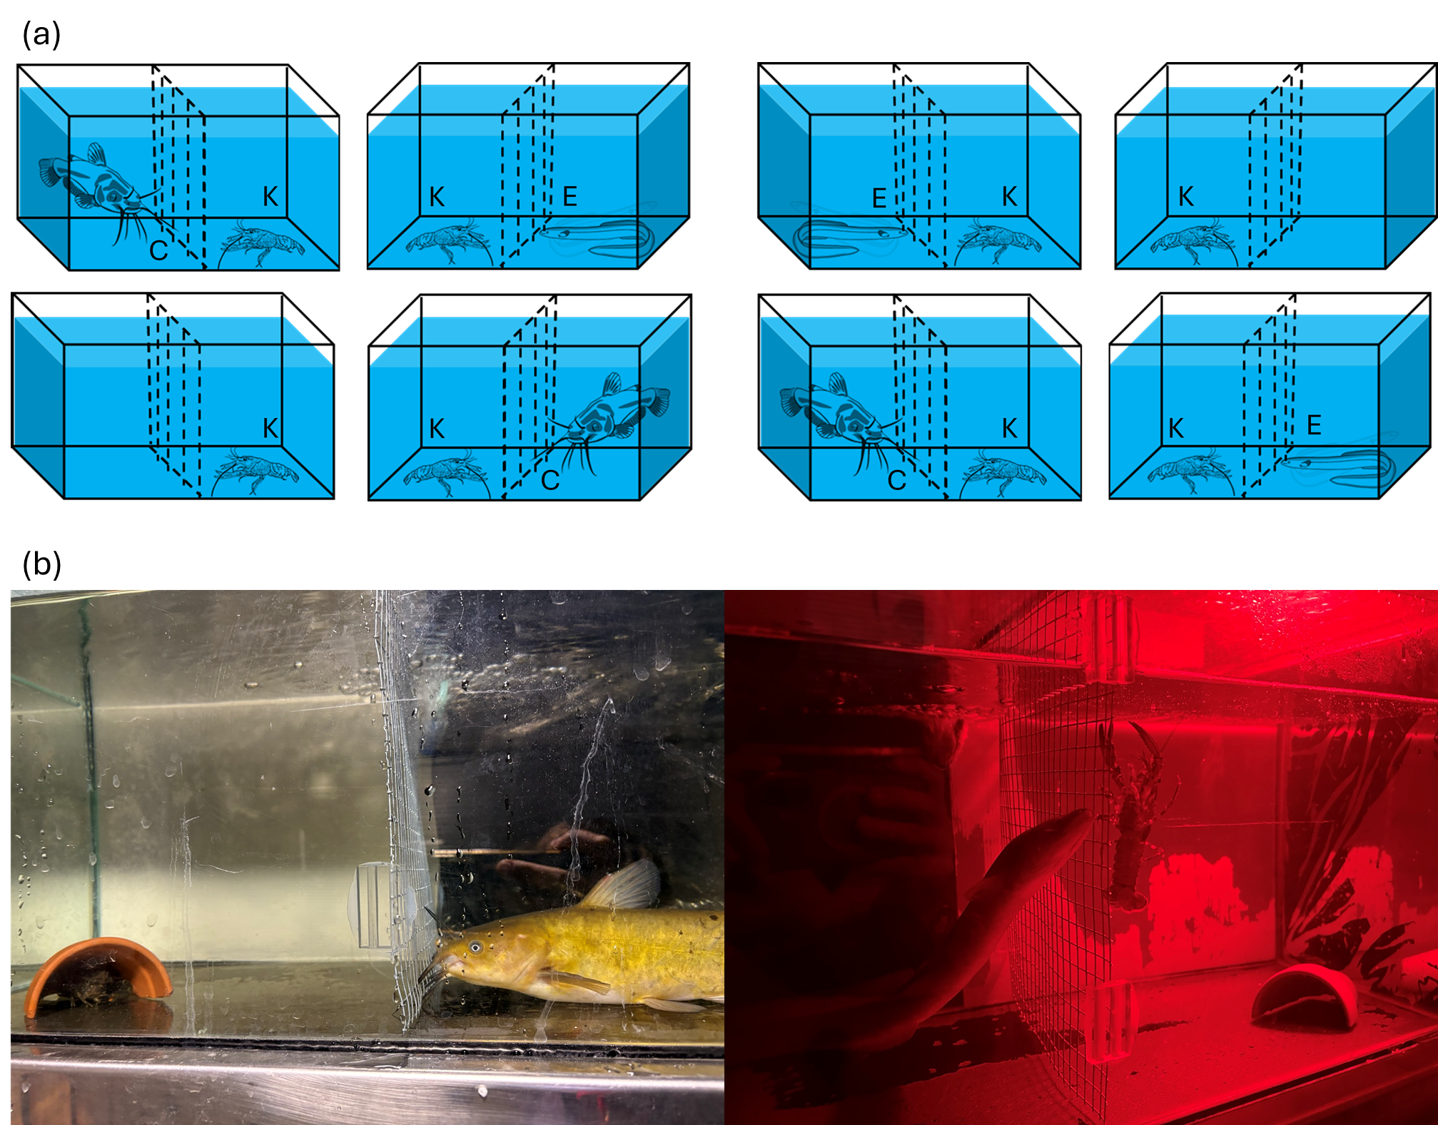
\includegraphics[keepaspectratio]{images/setup_combined.png}}

}

\caption{\label{fig-1-aquarium-setup}(a) Aquarium layout for kōura
refuge seeking behaviour experiment. Each experimental round consisted
of eight aquaria run simultaneously. Each tank contained a single kōura
(K) and refuge (half terracotta plant pot) on one side of a mesh
divider. On the other side was either a single catfish (C), eel (E) or a
control with no fish. The mesh divider allowed visual and chemical cues
while preventing direct physical contact between tank occupants. (b)
Experiments were repeated in light and dark (red light), with
photographs showing a catfish in the light regime (left) and and an eel
in the dark regime (red light) (right) separated from kōura by mesh
dividers.}

\end{figure}%

\begin{figure}[H]

\centering{

\pandocbounded{
\includegraphics[keepaspectratio]{index_files/figure-latex/analysis-fig-2-emmeans-plot-output-1.png}}

}

\caption{\label{fig-2-emmeans-plot}Predicted marginal probabilities of
refuge use from the beta-binomial GLMM for each level of treatment,
light condition, and experimental period. Points represent
model-estimated marginal means averaged over other factors, with 95\%
confidence intervals shown as error bars. Different letters (a, b)
indicate statistically significant differences between groups within
each factor based on multiple comparison-adjusted pairwise comparisons.
The dashed line at 0.5 marks the threshold where kōura spend half their
time in refuge.}

\end{figure}%

\textsubscript{Source:
\href{https://OlivierRaven.github.io/https---github.com-OlivierRaven-NCE_Koura_catfish/analysis-preview.html\#cell-fig-2-emmeans-plot}{Analysis
Notebook}}

\begin{verbatim}
systemfonts and textshaping have been compiled with different versions of Freetype. Because of this, textshaping will not use the font cache provided by systemfonts
\end{verbatim}

\begin{figure}[H]

\centering{

\pandocbounded{
\includegraphics[keepaspectratio]{index_files/figure-latex/analysis-fig-3-refuge-plot-output-2.png}}

}

\caption{\label{fig-3-refuge-plot}Kōura refuge use over the course of
the experiment, showing the proportion of time spent in refuge across
three periods (before, during, and after predator exposure) for each
treatment (catfish: dark grey solid line; eel: medium grey dashed line;
control: light grey dot-dash line) under light (top) and dark (bottom)
conditions. Black dashed vertical lines indicate the start and end of
predator exposure and grey vertical lines show individual observation
times.}

\end{figure}%

\textsubscript{Source:
\href{https://OlivierRaven.github.io/https---github.com-OlivierRaven-NCE_Koura_catfish/analysis-preview.html\#cell-fig-3-refuge-plot}{Analysis
Notebook}}

\begin{figure}[H]

\centering{

\pandocbounded{
\includegraphics[keepaspectratio]{index_files/figure-latex/analysis-fig-4-feeding-plot-output-2.png}}

}

\caption{\label{fig-4-feeding-plot}Mean kōura feeding rate (pellets
consumed per gram body weight ± SE) across predator treatments (catfish,
eel, control) and starvation periods (0, 3, and 4 days). Points
represent treatment means and error bars show standard error.}

\end{figure}%

\textsubscript{Source:
\href{https://OlivierRaven.github.io/https---github.com-OlivierRaven-NCE_Koura_catfish/analysis-preview.html\#cell-fig-4-feeding-plot}{Analysis
Notebook}}

\section*{Supplementary information}\label{supplementary-information}
\addcontentsline{toc}{section}{Supplementary information}

\begin{table}

\caption{\label{tbl-s1-refuge-prop}Proportion of kōura observations
recorded in refuge across experimental treatments (catfish, eel,
control), light conditions (light, dark), and periods (before, during,
and after predator exposure). Combined rows summarise across all levels
of a given factor. Values represent the proportion of total observations
where kōura were located in the refuge.}

\centering{

\begin{verbatim}
Unable to display output for mime type(s): text/html
\end{verbatim}

}

\end{table}%

\textsubscript{Source:
\href{https://OlivierRaven.github.io/https---github.com-OlivierRaven-NCE_Koura_catfish/analysis-preview.html\#cell-tbl-s1-refuge-prop}{Analysis
Notebook}}

{

\begin{longtable}[]{@{}lrrrr@{}}

\caption{\label{tbl-s2-feeding-anova}Type III ANOVA table for the linear
model of kōura feeding rate (pellets consumed per gram body weight).
Treatment and starvation period included as fixed effects.}

\tabularnewline

\toprule\noalign{}
Term & Sum Sq & Df & F value & p value \\
\midrule\noalign{}
\endhead
\bottomrule\noalign{}
\endlastfoot
(Intercept) & 0.014 & 1 & 1.734 & 0.195 \\
treatment & 0.018 & 2 & 1.133 & 0.332 \\
day\_starve & 0.137 & 2 & 8.632 & 0.001 \\
Residuals & 0.327 & 41 & NA & NA \\

\end{longtable}

}

\textsubscript{Source:
\href{https://OlivierRaven.github.io/https---github.com-OlivierRaven-NCE_Koura_catfish/analysis-preview.html\#cell-tbl-s2-feeding-anova}{Analysis
Notebook}}

\protect\phantomsection\label{refs}
\begin{CSLReferences}{1}{0}
\bibitem[\citeproctext]{ref-Abrams2000}
Abrams, P. A. (2000). The evolution of predator-prey interactions:
Theory and evidence. \emph{Annual Review of Ecology and Systematics},
\emph{31}(1), 79--105.
\url{https://doi.org/10.1146/annurev.ecolsys.31.1.79}

\bibitem[\citeproctext]{ref-Achtymichuk2025}
Achtymichuk, G. H., Fish, K. M., \& Ferrari, M. C. O. (2025). The power
of concentration: Antipredator responses to diluted frozen crayfish
alarm cues provide insights on ecologically relevant concentrations and
updates to methodology. \emph{PLOS One}, \emph{20}(12), e0340001.
\url{https://doi.org/10.1371/journal.pone.0340001}

\bibitem[\citeproctext]{ref-Adams2007}
Adams, S. B. (2007). Direct and indirect effects of channel catfish
(ictalurus punctatus) on native crayfishes (cambaridae) in experimental
tanks. \emph{The American Midland Naturalist}, \emph{158}(1), 85--96.
\url{https://doi.org/10.1674/0003-0031(2007)158\%5B85:daieoc\%5D2.0.co;2}

\bibitem[\citeproctext]{ref-Barnes2003}
Barnes, G. E., \& Hicks, B. J. (2003). \emph{Brown bullhead catfish
(ameiurus nebulosus) in lake taupo (managing invasive freshwater fish in
new zealand)}. Department of Conservation.

\bibitem[\citeproctext]{ref-Beattie2018}
Beattie, M. C., \& Moore, P. A. (2018). Predator recognition of chemical
cues in crayfish: Diet~and experience influence the ability
to~detect~predation~threats. \emph{Behaviour}, \emph{155}(6), 505--530.
\url{https://doi.org/10.1163/1568539x-00003501}

\bibitem[\citeproctext]{ref-Blake1993}
Blake, M. A., \& Hart, P. J. B. (1993). The behavioural responses of
juvenile signal crayfish pacifastacus leniusculus to stimuli from perch
and eels. \emph{Freshwater Biology}, \emph{29}(1), 89--97.
\url{https://doi.org/10.1111/j.1365-2427.1993.tb00747.x}

\bibitem[\citeproctext]{ref-Bronmark2012}
Brönmark, C., \& Hansson, L.-A. (2012). \emph{Chemical ecology in
aquatic systems}. Oxford University Press.

\bibitem[\citeproctext]{ref-Brooks2017}
Brooks, E., Mollie, Kristensen, K., Benthem, J., Koen, Magnusson, A.,
Berg, W., Casper, Nielsen, A., Skaug, J., Hans, Mächler, M., \& Bolker,
M., Benjamin. (2017). glmmTMB balances speed and flexibility among
packages for zero-inflated generalized linear mixed modeling. \emph{The
R Journal}, \emph{9}(2), 378. \url{https://doi.org/10.32614/rj-2017-066}

\bibitem[\citeproctext]{ref-Brown2004}
Brown, G. E., Poirier, J.-F., \& Adrian, J. C. (2004). Assessment of
local predation risk: The role of subthreshold concentrations of
chemical alarm cues. \emph{Behavioral Ecology}, \emph{15}(5), 810--815.
\url{https://doi.org/10.1093/beheco/arh084}

\bibitem[\citeproctext]{ref-Brown2009}
Brown, L. A. (2009). \emph{Habitat determinants and predatory
interactions of the endemic freshwater crayfish (koura, paranephrops
planifrons) in the lower north island, new zealand} {[}Massey
University{]}. \url{http://hdl.handle.net/10179/1168}

\bibitem[\citeproctext]{ref-Burnham2002}
Burnham, K. P., \& Anderson, D. R. (2002). (pp. 267--351). Springer New
York. \url{https://doi.org/10.1007/978-0-387-22456-5_6}

\bibitem[\citeproctext]{ref-Carthey2014}
Carthey, A. J. R., \& Banks, P. B. (2014). Naïveté in novel ecological
interactions: Lessons from theory and experimental evidence.
\emph{Biological Reviews}, \emph{89}(4), 932--949.
\url{https://doi.org/10.1111/brv.12087}

\bibitem[\citeproctext]{ref-Clinchy2013}
Clinchy, M., Sheriff, M. J., \& Zanette, L. Y. (2012). Predator‐induced
stress and the ecology of fear. \emph{Functional Ecology}, \emph{27}(1),
56--65. \url{https://doi.org/10.1111/1365-2435.12007}

\bibitem[\citeproctext]{ref-Collier1997}
Collier, K. J., Parkyn, S. M., \& Rabeni, C. F. (1997). Koura: A
keystone species. \emph{Water and Atmosphere}, \emph{5}(1), 18--20.

\bibitem[\citeproctext]{ref-Dawkins1979}
Dawkins, R., \& Krebs, J. R. (1979). Arms races between and within
species. \emph{Proceedings of the Royal Society of London. B. Biological
Sciences}, \emph{205}(1161), 489--511.
\url{https://doi.org/10.1098/rspb.1979.0081}

\bibitem[\citeproctext]{ref-Dedual2019}
Dedual, M. (2019). \emph{Summary of the impacts and control methods of
brown bullhead catfish (ameiurus nebulosus lesueur 1815) in new zealand
and overseas}. Bay of Plenty Regional Council.
\url{https://atlas.boprc.govt.nz/api/v1/edms/document/A3591759/content}

\bibitem[\citeproctext]{ref-Devcich1979}
Devcich, A. A. (1979). \emph{An ecological study of paranephrops
planifrons white (decapoda: Parastacidae) in lake rotoiti, north island}
{[}PhD thesis{]}. University of Waikato.

\bibitem[\citeproctext]{ref-Doherty2016}
Doherty, T. S., Glen, A. S., Nimmo, D. G., Ritchie, E. G., \& Dickman,
C. R. (2016). Invasive predators and global biodiversity loss.
\emph{Proceedings of the National Academy of Sciences}, \emph{113}(40),
11261--11265. \url{https://doi.org/10.1073/pnas.1602480113}

\bibitem[\citeproctext]{ref-Ehlman2019}
Ehlman, S. M., Trimmer, P. C., \& Sih, A. (2019). Prey responses to
exotic predators: Effects of old risks and new cues. \emph{The American
Naturalist}, \emph{193}(4), 575--587.
\url{https://doi.org/10.1086/702252}

\bibitem[\citeproctext]{ref-Figler2005}
Figler, M. H., Blank, G. S., \& Peeke, H. V. S. (2005). Shelter
competition between resident male red swamp crayfish procambarus clarkii
(girard) and conspecific intruders varying by sex and reproductive
status. \emph{Marine and Freshwater Behaviour and Physiology},
\emph{38}(4), 237--248. \url{https://doi.org/10.1080/10236240500376477}

\bibitem[\citeproctext]{ref-Fox2018}
Fox, J., \& Weisberg, S. (2018). \emph{An r companion to applied
regression}. SAGE Publications.

\bibitem[\citeproctext]{ref-Gherardi2011}
Gherardi, F., Mavuti, K. M., Pacini, N., Tricarico, E., \& Harper, D. M.
(2011). The smell of danger: Chemical recognition of fish predators by
the invasive crayfish procambarus clarkii. \emph{Freshwater Biology},
\emph{56}(8), 1567--1578.
\url{https://doi.org/10.1111/j.1365-2427.2011.02595.x}

\bibitem[\citeproctext]{ref-Hartig2024}
{Hartig, F., Lohse, L., \& leite, M. de S.} (2024). \emph{DHARMa:
Residual diagnostics for hierarchical (multi-level / mixed) regression
models} (Version 0.4.7) {[}Computer software{]}.
\url{https://cran.r-project.org/web/packages/DHARMa/index.html}

\bibitem[\citeproctext]{ref-Hazlett2003}
Hazlett, B. A. (2003). The effects of starvation on crayfish responses
to alarm odor. \emph{Ethology}, \emph{109}(7), 587--592.
\url{https://doi.org/10.1046/j.1439-0310.2003.00902.x}

\bibitem[\citeproctext]{ref-Hicks1997}
Hicks, B. J. (1997). Food webs in forest and pasture streams in the
waikato region, new zealand: A study based on analyses of stable
isotopes of carbon and nitrogen, and fish gut contents. \emph{New
Zealand Journal of Marine and Freshwater Research}, \emph{31}(5),
651--664. \url{https://doi.org/10.1080/00288330.1997.9516796}

\bibitem[\citeproctext]{ref-Johnson2014}
Johnson, M. F., Rice, S. P., \& Reid, I. (2014). The activity of signal
crayfish (pacifastacus leniusculus) in relation to thermal and hydraulic
dynamics of an alluvial stream, UK. \emph{Hydrobiologia}, \emph{724}(1),
41--54. \url{https://doi.org/10.1007/s10750-013-1708-1}

\bibitem[\citeproctext]{ref-Kindlinger2017}
Kindinger, T. L., \& Albins, M. A. (2017). Consumptive and
non-consumptive effects of an invasive marine predator on native
coral-reef herbivores. \emph{Biological Invasions}, \emph{19}(1),
131--146. \url{https://doi.org/10.1007/s10530-016-1268-1}

\bibitem[\citeproctext]{ref-Kusabsinrevision}
Kusabs, I. A., Duggan, I. C., Scholes, P., Bruere, A., Te Kurapa, T. W.,
Grant, T., \& Burdon, F. J. (n.d.). Invasive catfish linked to the
decline of freshwater crayfish in two aotearoa new zealand lakes.
\emph{Manuscript Submitted for Publication}.

\bibitem[\citeproctext]{ref-Kusabs2009}
Kusabs, I. A., \& Quinn, J. M. (2009). Use of a traditional maori
harvesting method, the tau kōura, for monitoring kōura (freshwater
crayfish, paranephrops planifrons) in lake rotoiti, north island, new
zealand. \emph{New Zealand Journal of Marine and Freshwater Research},
\emph{43}(3), 713--722. \url{https://doi.org/10.1080/00288330909510036}

\bibitem[\citeproctext]{ref-Laundre2001}
Laundré, J. W., Hernández, L., \& Altendorf, K. B. (2001). Wolves, elk,
and bison: Reestablishing the {``landscape of fear''} in yellowstone
national park, u.s.a. \emph{Canadian Journal of Zoology}, \emph{79}(8),
1401--1409. \url{https://doi.org/10.1139/z01-094}

\bibitem[\citeproctext]{ref-Lee2025}
Lee, F., Kusabs, I. A. K., Perry, G. L. W., \& MacNeil, C. (2025).
Identifying refugia from the synergistic threats of climate change and
invasive species. \emph{Web Ecology}, \emph{25}(2), 221--239.
\url{https://doi.org/10.5194/we-25-221-2025}

\bibitem[\citeproctext]{ref-Lenth2026}
Lenth, R. V., Piaskowski, J., Banfai, B., Bolker, B., Buerkner, P.,
Giné-Vázquez, I., Hervé, M., Jung, M., Love, J., Miguez, F., Riebl, H.,
\& Singmann, H. (2026). \emph{Emmeans: Estimated marginal means, aka
least-squares means} (Version 2.0.2) {[}Computer software{]}.
\url{https://cran.r-project.org/web/packages/emmeans/index.html}

\bibitem[\citeproctext]{ref-Lima1990}
Lima, S. L., \& Dill, L. M. (1990). Behavioral decisions made under the
risk of predation: A review and prospectus. \emph{Canadian Journal of
Zoology}, \emph{68}(4), 619--640. \url{https://doi.org/10.1139/z90-092}

\bibitem[\citeproctext]{ref-MacNeil2025}
MacNeil, C., Lee, F., Kusabs, I., \& Holmes, R. (2025). The biter bit;
scavenging behaviour of native freshwater crayfish on the carrion of
native and introduced fish predators in aotearoa-new zealand.
\emph{Knowledge \& Management of Aquatic Ecosystems}, (426), 29.
\url{https://doi.org/10.1051/kmae/2025022}

\bibitem[\citeproctext]{ref-Martin2014}
Martin, C. W. (2014). Naïve prey exhibit reduced antipredator behavior
and survivorship. \emph{PeerJ}, \emph{2}, e665.
\url{https://doi.org/10.7717/peerj.665}

\bibitem[\citeproctext]{ref-McDowall1990}
McDowall, R. M. (1990). \emph{New zealand freshwater fishes: A natural
history and guide}.
\url{https://agris.fao.org/search/en/providers/122621/records/6473966cce9437aa76003d0e}

\bibitem[\citeproctext]{ref-Nystrom2005}
Nyström, P. (2005). Non‐lethal predator effects on the performance of a
native and an exotic crayfish species. \emph{Freshwater Biology},
\emph{50}(12), 1938--1949.
\url{https://doi.org/10.1111/j.1365-2427.2005.01438.x}

\bibitem[\citeproctext]{ref-Parkyn2001}
Parkyn, S. M., Collier, K. J., \& Hicks, B. J. (2001). New zealand
stream crayfish: Functional omnivores but trophic predators?
\emph{Freshwater Biology}, \emph{46}(5), 641--652.
\url{https://doi.org/10.1046/j.1365-2427.2001.00702.x}

\bibitem[\citeproctext]{ref-Peacor2001}
Peacor, S. D., \& Werner, E. E. (2001). The contribution of
trait-mediated indirect effects to the net effects of a predator.
\emph{Proceedings of the National Academy of Sciences}, \emph{98}(7),
3904--3908. \url{https://doi.org/10.1073/pnas.071061998}

\bibitem[\citeproctext]{ref-Preisser2005}
Preisser, E. L., Bolnick, D. I., \& Benard, M. F. (2005). Scared to
death? The effects of intimidation and consumption in predator--prey
interactions. \emph{Ecology}, \emph{86}(2), 501--509.
\url{https://doi.org/10.1890/04-0719}

\bibitem[\citeproctext]{ref-Preisser2008}
Preisser, E. L., \& Bolnick, D. I. (2008). The many faces of fear:
Comparing the pathways and impacts of nonconsumptive predator effects on
prey populations. \emph{PLoS ONE}, \emph{3}(6), e2465.
\url{https://doi.org/10.1371/journal.pone.0002465}

\bibitem[\citeproctext]{ref-RCoreTeam2025}
R Core Team. (2025). \emph{R: A language and environment for statistical
computing} {[}Computer software{]}. R Foundation for Statistical
Computing. \url{https://www.R-project.org/}

\bibitem[\citeproctext]{ref-RambergPihl2020}
Ramberg-Pihl, N. C., \& Yurewicz, K. L. (2020). Behavioral responses of
northern crayfish (faxonius virilis) to conspecific alarm cues and
predator cues from smallmouth bass (micropterus dolomieu). \emph{Marine
and Freshwater Behaviour and Physiology}, \emph{53}(1), 1--16.
\url{https://doi.org/10.1080/10236244.2020.1717338}

\bibitem[\citeproctext]{ref-Ryan2009}
Ryan, P. (2009). \emph{Eels \textbar{} te ara encyclopedia of new
zealand}. \url{https://teara.govt.nz/en/eels}

\bibitem[\citeproctext]{ref-Schmitz1997}
Schmitz, O. J., Beckerman, A. P., \& O'Brien, K. M. (1997). Behaviorally
mediated trophic cascades: Effects of predation risk on food web
interactions. \emph{Ecology}, \emph{78}(5), 1388--1399.
\url{https://doi.org/10.1890/0012-9658(1997)078\%5B1388:bmtceo\%5D2.0.co;2}

\bibitem[\citeproctext]{ref-Scott1973}
Scott, W. B., \& Crossman, E. J. (1973). \emph{Freshwater fishes of
canada}. Fisheries Research Board of Canada.

\bibitem[\citeproctext]{ref-Shave1994}
Shave, Cathy. R., Townsend, C. R., \& Crowl, T. A. (1994). Anti-predator
behaviours of a freshwater crayfish (paranephrops zealandicus) to a
native and an introduced predator. \emph{New Zealand Journal of
Ecology}, \emph{18}(1), 1--10.

\bibitem[\citeproctext]{ref-Sheriff2020}
Sheriff, M. J., Peacor, S. D., Hawlena, D., \& Thaker, M. (2020).
Non-consumptive predator effects on prey population size: A dearth of
evidence. \emph{Journal of Animal Ecology}, \emph{89}(6), 1302--1316.
\url{https://doi.org/10.1111/1365-2656.13213}

\bibitem[\citeproctext]{ref-Sih2010}
Sih, A., Bolnick, D. I., Luttbeg, B., Orrock, J. L., Peacor, S. D.,
Pintor, L. M., Preisser, E., Rehage, J. S., \& Vonesh, J. R. (2010).
Predator--prey naïveté, antipredator behavior, and the ecology of
predator invasions. \emph{Oikos}, \emph{119}(4), 610--621.
\url{https://doi.org/10.1111/j.1600-0706.2009.18039.x}

\bibitem[\citeproctext]{ref-Sih2023}
Sih, A., Chung, H. J., Neylan, I., Ortiz-Jimenez, C., Sakai, O., \&
Szeligowski, R. (2023). Fear generalization and behavioral responses to
multiple dangers. \emph{Trends in Ecology \& Evolution}, \emph{38}(4),
369--380. \url{https://doi.org/10.1016/j.tree.2022.11.001}

\bibitem[\citeproctext]{ref-Sih2011}
Sih, A., Ferrari, M. C. O., \& Harris, D. J. (2011). Evolution and
behavioural responses to human‐induced rapid environmental change.
\emph{Evolutionary Applications}, \emph{4}(2), 367--387.
\url{https://doi.org/10.1111/j.1752-4571.2010.00166.x}

\bibitem[\citeproctext]{ref-Smee2006}
Smee, D. L., \& Weissburg, M. J. (2006). Hard clams (mercenaria
mercenaria) evaluate predation risk using chemical signals from
predators and injured conspecifics. \emph{Journal of Chemical Ecology},
\emph{32}(3), 605--619. \url{https://doi.org/10.1007/s10886-005-9021-8}

\bibitem[\citeproctext]{ref-Sniegula2025}
Sniegula, S., Konczarek, D., Bonk, M., Antoł, A., Amer, N. R., \& Stoks,
R. (2025). Non-consumptive effects of native, alien and invasive alien
crayfish on damselfly egg life history and carry-over effects on larval
physiology. \emph{NeoBiota}, \emph{97}, 215--235.
\url{https://doi.org/10.3897/neobiota.97.139760}

\bibitem[\citeproctext]{ref-Stebbing2010}
Stebbing, P. D., Watson, G. J., \& Bentley, M. G. (2010). The response
to disturbance chemicals and predator odours of juvenile and adult
signal crayfish pacifastacus leniusculus (dana). \emph{Marine and
Freshwater Behaviour and Physiology}, \emph{43}(3), 183--195.
\url{https://doi.org/10.1080/10236244.2010.487301}

\bibitem[\citeproctext]{ref-Stein1976}
Stein, R. A., \& Magnuson, J. J. (1976). Behavioral response of crayfish
to a fish predator. \emph{Ecology}, \emph{57}(4), 751--761.
\url{https://doi.org/10.2307/1936188}

\bibitem[\citeproctext]{ref-Usio2004}
Usio, N., \& Townsend, C. R. (2004). Roles of crayfish: Consequences of
predation and bioturbation for stream invertebrates. \emph{Ecology},
\emph{85}(3), 807--822. \url{https://doi.org/10.1890/02-0618}

\bibitem[\citeproctext]{ref-Wood2020a}
Wood, T. C., \& Moore, P. A. (2020a). Big and bad: How relative predator
size and dietary information influence rusty crayfish (faxonius
rusticus) behavior and resource-use decisions. \emph{Canadian Journal of
Zoology}, \emph{98}(1), 62--72.
\url{https://doi.org/10.1139/cjz-2019-0089}

\bibitem[\citeproctext]{ref-Wood2020b}
Wood, T. C., \& Moore, P. A. (2020b). Fine-tuned responses to chemical
landscapes: Crayfish use predator odors to assess threats based on
relative size ratios. \emph{Ecosphere}, \emph{11}(9), e03188.
\url{https://doi.org/10.1002/ecs2.3188}

\bibitem[\citeproctext]{ref-Wright2010}
Wright, T. F., Eberhard, J. R., Hobson, E. A., Avery, M. L., \&
Russello, M. A. (2010). Behavioral flexibility and species invasions:
The adaptive flexibility hypothesis. \emph{Ethology Ecology \&
Evolution}, \emph{22}(4), 393--404.
\url{https://doi.org/10.1080/03949370.2010.505580}

\bibitem[\citeproctext]{ref-Zhao2024}
Zhao, M., Feng, G., Wang, H., Shen, C., Fu, Y., Zhang, Y., Zhang, H.,
Yao, Y., Chen, J., \& Xu, W. (2024). The influence of shelter type and
coverage on crayfish (procambarus clarkii) predation by catfish (silurus
asotus): A controlled environment study. \emph{Animals}, \emph{14}(8),
1147. \url{https://doi.org/10.3390/ani14081147}

\end{CSLReferences}




\end{document}
